\documentclass[conference]{IEEEtran}
\IEEEoverridecommandlockouts
% The preceding line is only needed to identify funding in the first footnote. If that is unneeded, please comment it out.

\usepackage[bahasa]{babel}

\usepackage[noadjust]{cite}
\usepackage{amsmath,amssymb,amsfonts}
\usepackage{algorithmic}
\usepackage{graphicx}
\usepackage{textcomp}
\usepackage{multirow}
\usepackage[table]{xcolor}

\def\BibTeX{{\rm B\kern-.05em{\sc i\kern-.025em b}\kern-.08em
    T\kern-.1667em\lower.7ex\hbox{E}\kern-.125emX}}
\begin{document}

\title{Peningkatan Kinerja Modul Pencocokan Pola dalam Sistem Deteksi Intrusi Snort Menggunakan GPU}

\author{
\IEEEauthorblockN{Afrizal Fikri}
\IEEEauthorblockA{{School of Electrical Engineering and Informatics} \\
{Institut Teknologi Bandung}\\
{Bandung, Indonesia} \\
afrizalf96@gmail.com}
\and
\IEEEauthorblockN{Achmad Imam Kistijantoro}
\IEEEauthorblockA{{School of Electrical Engineering and Informatics} \\
{Institut Teknologi Bandung}\\
{Bandung, Indonesia} \\
imam@informatika.org}
}

\maketitle

\begin{abstract}
    Kemajuan teknologi telah memberikan berpengaruh pada pertumbuhan pesat penggunaan data digital. Di era digital ini, banyak transaksi penting juga dilakukan melalui dunia maya. Mayoritas dari itu adalah data konfidensial yang rahasia. Dengan demikian, jaminan keamanan menjadi sangat penting. Salah satu titik masuk dari penyalahgunaan data berasal dari sisi server. Penjaminan keamanan pada server yang menggunakan sistem deteksi intrusi jaringan (NIDS) dapat menghabiskan sumber daya dan waktu yang banyak. Salah satu bagian penting dari NIDS adalah pencocokan string dalam tahap analisis. Berdasarkan masalah ini, makalah ini akan membahas eksperimen untuk meningkatkan kecepatan pencocokan string untuk memaksimalkan kinerja keseluruhan sistem menggunakan GPU. Berdasarkan percobaan dan pengujian, solusi yang diusulkan memiliki waktu operasi yang jauh lebih baik dibandingkan dengan solusi CPU saat ini dengan tetap menjaga akurasi.
\end{abstract}

\begin{IEEEkeywords}
    pattern matching; intrusion detection; GPU; parallel computation; CUDA
\end{IEEEkeywords}

\section{Pendahuluan}

Salah satu sumber daya yang penting untuk dilindungi yaitu \emph{server}. Banyak aspek security yang terdapat pada \emph{server} dan dapat dengan mudah diserang \cite{owasp}. Solusi untuk pengamanan \emph{server} dari \emph{request} berbahaya adalah dengan menggunakan sistem deteksi intrusi jaringan atau \emph{network intrusion detection system} (NIDS). NIDS berfungsi mengenali kemungkinan serangan dari \emph{request} yang diterima pada \emph{server} atau \emph{client} sebagai tindakan pencegahan. Ketika \emph{request} dianggap berbahaya, maka dapat dilakukan tindakan lanjutan untuk mencegah kerusakan lebih lanjut pada aset. NIDS yang melakukan tindakan preventif seperti ini disebut juga NIPS (\emph{network intrusion prevention system}).

Karena adanya peningkatan kecepatan \emph{traffic} internet dan banyaknya serangan yang terjadi, maka dibutuhkan NIDS yang mampu melakukan deteksi dengan lebih cepat. Salah satu \emph{bottleneck} dalam pengecekan paket adalah banyaknya \emph{rule} yang harus dicocokkan \cite{pcre2007}. Sehingga, peningkatan secara signifikan dapat dicapai salah satunya dengan meningkatkan kemampuan komputasi untuk pencocokan banyak paket secara paralel. 

Komputasi paralel dapat dilakukan dengan \emph{multicore} CPU \cite{multi2004}, \emph{multicore} GPU \cite{gnort2008}, atau prosesor terkustomisasi seperti ASIC dan FPGA \cite{fpga2008}. Perbedaan antara CPU dan GPU adalah bagaimana mereka memproses pekerjaan \cite{cuda}. CPU didesain untuk melakukan komputasi secara serial dengan beberapa \emph{core}, sementara GPU dapat memiliki ribuan unit komputasi yang disebut \emph{stream processor} (SP) yang bekerja secara paralel.

Berdasarkan tinjauan di atas, penelitian ini akan membahas metode yang dapat digunakan dalam mempercepat pencocokan string pada NIDS dengan memanfaatkan \emph{multithreading} pada GPU. Pengujian akan dilakukan untuk mengukur peningkatan kinerja terhadap solusi CPU yang digunakan oleh NIDS saat ini.

\section{Pencocokan string}
Secara umum, ada dua jenis pencocokan string: \emph{single pattern string matching} dan \emph{multi pattern string matching}. Kami akan fokus ke pencocokan \emph{multi pattern string matching}. Ada beberapa algoritma terkenal untuk \emph{multi pattern string matching}, seperti algoritma Aho-Corasick \cite{ahoc1975}, Commentz-Walter \cite{walter1980}, dan Wu-Manber \cite{wu92}. Implementasi akan berbasis variasi dari algoritma Aho-Corasick.

    \subsection{Algoritma Aho-Corasick}
    Algoritma Aho-Corasick adalah jenis algoritma pencocokan string yang bekerja dengan mencocokkan tiap string ke kamus. Kamus akan berisi semua pola untuk dicocokkan dalam bentuk \emph{state machine}.
    
    Dalam algoritma ini, operasi pencocokan dilakukan dengan menelusuri \emph{state machine} untuk tiap karakter dalam string input. Jika sampai pada \emph{final state}, maka string input dianggap cocok dengan salah satu pola. Pencocokan berlanjut hingga string input berakhir. 

    \begin{figure}[htbp]
        \centerline{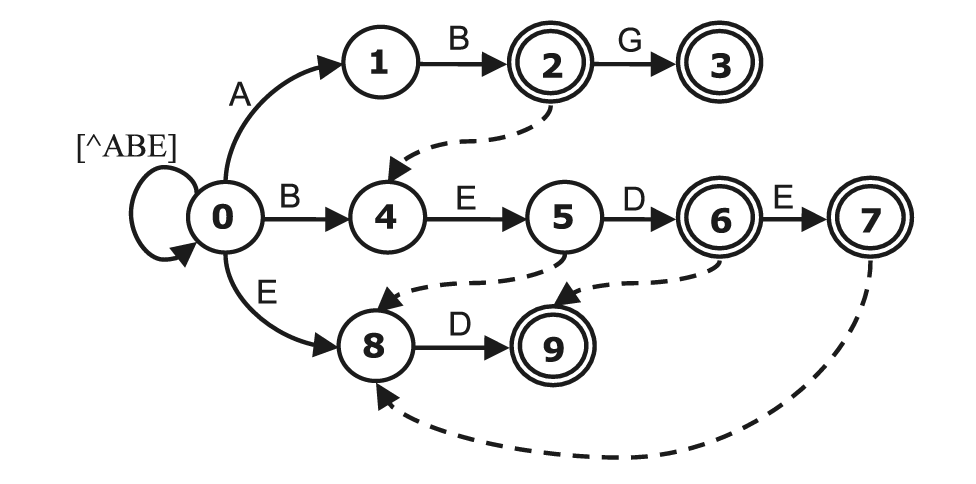
\includegraphics[width=0.4\textwidth]{../src/resources/aho-c.png}}
        \caption{Example state machine of Aho-Corasick dictionary.}
    \end{figure}

    Aho-Corasick menggunakan \emph{failure function} untuk melakukan \emph{backtrack} setelah berhenti di salah satu \emph{final state}. \emph{Failure function} akan menunjuk dari \emph{final state} sekarang ke prefiks pola terpanjang yang cocok dengan sufiks dari pola yang saat ini dicocokkan \cite{ahoc1975}. \emph{Failure function} mengurangi redundansi untuk sekuens yang telah dilewati. Dengan metode ini, semua pola yang ada dalam kalimat dapat dicocokkan dengan sekali penelusuran dan mengurangi kompleksitas dari $O(mn)$ to $O(n)$. 

    Dalam algoritma ini, akses memori menjadi \emph{bottleneck}. Setiap operasi penelusuran akan mengambil satu entri dari tabel. Karena akses memori lebih mahal daripada komputasi, algoritma ini terbatas dengan memori (\emph{memory bound}) \cite{lin2013}.

    \subsection{Data Parallel Aho-Corasick}
    Untuk membuat Aho-Corasick menjadi \emph{multithreading}, beban pencocokan perlu dibagi ke setiap \emph{thread}. Salah satu caranya adalah dengan mempartisi input menjadi beberapa segmen dan kemudian setiap \emph{thread} akan mencocokkan tiap segmen yang berkorespondensi terhadap kamus. Namun, jika ada pola yang menjangkau beberapa segmen sekaligus, pola tidak akan dikenali pada kedua \emph{thread}. Masalah ini dikenal sebagai \emph{boundary matching problem}. Sehingga perlu memperpanjang sesuai dengan panjang pola terpanjang. Akses memori meningkat menjadi $O((n/s + m) * s) = O(n + ms)$ dengan $s$ adalah banyak segmen. 

    \begin{figure}[htbp]
        \centerline{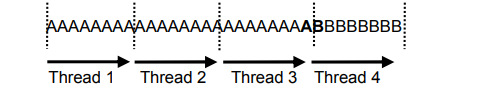
\includegraphics[width=0.4\textwidth]{../src/resources/boundary.png}}
        \caption{Pattern \textbf{AB} not recognized by both thread 3 and 4}
    \end{figure}

    \subsection{Parallel Failureless Aho-Corasick}
    Metode lain untuk mengadaptasi Aho-Corasick dengan \emph{multithreading} adalah membagi \emph{thread} ke semua \emph{byte} karakter. Setiap \emph{thread} akan mencocokkan pola yang dimulai dengan karakter yang berkorespondensi dan selesai ketika ada \emph{final state} atau tidak ada transisi yang valid pada karakter \cite{lin2013}. Konsekuensinya adalah setiap \emph{thread} paling banyak hanya akan cocok dengan satu pola.
    
    Dengan demikian, \emph{failure function} tidak diperlukan lagi. Selain itu, \emph{boundary matching problem} tidak akan terjadi dengan menggunakan pendekatan ini. Pendekatan ini dinamakan juga sebagai \emph{parallel failureless Aho-Corasick} (PFAC).

    \begin{figure}[htbp]
        \centerline{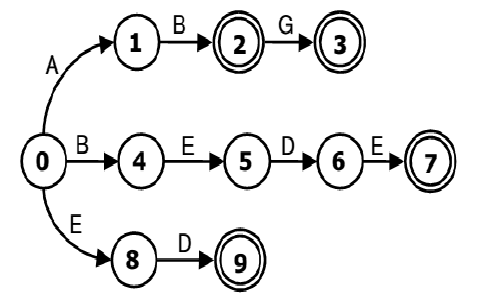
\includegraphics[width=0.4\textwidth]{../src/resources/pfac.png}}
        \caption{State machine without failure function}
    \end{figure} 

\section{Related Works}

    \subsection{Utilization of Double Buffering Scheme, Texture Memory and Pinned Memory}

        Dalam tulisan ini, implementasi pencocokan berbasis GPU telah diusulkan menggunakan algoritma Aho-Corasick. Selain pemanfaatan GPU multithreading, ada beberapa penyesuaian untuk mengimpor Aho-Corasick ke GPGPU. Mesin negara dibangun menggunakan tabel transisi pada tabel 2D pada memori tekstur. Berdasarkan eksperimen, penerapan ini meningkatkan kinerja sebesar 19\% \cite{gnort2008}.
        
        Untuk skema transfer memori, skema \emph{double buffering} diusulkan. Paket akan di-batch dalam satu \emph{buffer}. Setiap kali \emph{buffer} penuh, semua paket ditransfer ke GPU dalam satu operasi. Mentransfer dari \emph{perangkat} ke \emph{host} juga dilakukan dengan cara yang sama. Semua hasil akan dikumpulkan di \emph{buffer} kedua dan ditransfer ketika penuh.
        
        Trik optimasi lain yang digunakan adalah menggunakan \emph{pinned memory}. Kedua \emph{buffer} in \emph{host} akan manggunanakan \emph{pinned memory} untuk mengurangi swappiness. Dan juga \emph{pinned memory} memungkinkan transfer secara langsung tanpa melalui CPU atau \emph{direct memory access} (DMA) dan mengurangi kebutuhan komputasi dan latensi. Desain ini dapat meningkatkan kinerja sistem hingga 3,2 kali lebih tinggi daripada implementasi menggunakan \emph{multithreading} pada CPU.

    \subsection{Scalable Architecture for Maximizing GPU Utilization}

        Dengan profiling, disimpulkan bahwa \emph{bottleneck} terjadi pada 3 komponen: akuisisi paket, pencocokan string, dan pencocokan aturan opsi oleh \emph{regular expression}. Selain itu, khususnya di dalam komponen pencocokan string, rata-rata utilisasi GPU masih rendah. Penelitian ini mencoba menerapkan perbaikan arsitektur pada NIDS. Diantara metode yang diusulkan adalah \emph{pipelining} dan \emph{payload batching}. \emph{Pipelining} digunakan untuk memisahkan penggunaan \emph{thread} untuk transfer dan pencocokan. Dan dengan arsitektur ini, NIDS dapat ditingkatkan ke beberapa GPU dan CPU \emph{core} inti \cite{kargus2012}.
        
        Perbaikan yang dicapai dengan metode ini adalah sekitar 1,5 hingga 4 kali lebih baik dibandingkan dengan solusi \emph{baseline} Snort. Evaluasi dilakukan menggunakan CPU ganda Intel X5680 dengan masing-masing 12 core dan GPU ganda NVIDIA GTX 580. NIDS dijalankan di bawah \emph{traffic} jaringan dengan kapasitas sekitar 40 Gbps dan bisa mencapai \emph{throughput} 25,2 Gbps.

    \subsection{Failureless Aho-Corasick by Maximizing Shared Memory Usage}

        Salah satu cara untuk melakukan pencocokan Aho-Corasick adalah dengan menetapkan setiap \emph{byte} input ke setiap \emph{thread} secara bersamaan. Kemudian setiap \emph{thread} akan melakukan pencocokan yang dimulai dengan \emph{byte} yang ditetapkan. Pencocokan berhenti setiap kali masuk \emph{final state} atau transisi valid tidak ada. Pendekatan ini tidak memerlukan \emph{failure function}. Sehingga setiap \emph{thread} hanya bertanggung jawab untuk mencocokkan paling banyak satu pola \cite{lin2013}.
        
        Pendekatan baru ini memanfaatkan \emph{memory coaelescing} dalam GPU sehingga \emph{byte} yang berurutan dapat dimuat sekaligus. Untuk lebih meningkatkan kinerja, transisi dari \emph{state} awal akan dimuat ke \emph{shared memory} untuk mengurangi transaksi ke \emph{global memory}.
        
        Karena tabel transisi dapat sangat besar, \emph{shared memory} tidak dapat menampung tabel transisi. Sehingga, sebagai alternatif untuk tabel transisi akan diikat ke \emph{texture memory}. \emph{Texture memory} memiliki beberapa kelebihan seperti memiliki \emph{cache} lebih besar dan cocok untuk melakukan akses dengan pola akses yang sulit diprediksi. Pengujian menggunakan dataset PCAP dari DEFCON menunjukkan peningkatan kinerja yang signifikan. Menggunakan CPU Intel Core i7-950 dan GPU NVIDIA GTX 580, \emph{throughput} sistem bisa menjadi 3 kali dibandingkan dengan Snort \emph{baseline}.

\section{Proposed Solution}
    \subsection{Matching Algorithm}
        Untuk mengimplementasikan Aho-Corasick ke GPU, kita perlu mengeksploitasi SIMD (\emph{single instruction multiple data}) secara optimal. Pendekatan data paralel adalah salah satu pendekatan yang paling mudah untuk diterapkan. Masukan ada dipartisi menjadi beberapa segmen. Setelah memisahkan segmen, masing-masing segmen akan dijalankan di \emph{thread} berbeda dengan ekstensi sepanjang pola terpanjang. Pendekatan ini memiliki 2 masalah: ekstensi meningkatkan transaksi data secara drastis, dan tidak optimal jika masukan dipisah menjadi banyak segmen. GPU dapat membangkitkan ratusan \emph{thread} dan dengan demikian semua \emph{thread} dapat dimanfaatkan secara optimal.
        
        Alternatif lain adalah dengan menggunakan metode yang disebut PFAC. Ide mengalokasikan tiap \emph{thread} ke setiap \emph{byte} dari aliran input memiliki implikasi penting pada efisiensi \emph{state machine} PFAC.

        \begin{enumerate}
            \item 
            Tiap \emph{thread} hanya bertanggung jawab dengan string yang dimulai dengan karakter pada \emph{thread} tersebut. Ketika tidak ada pola yang cocok dengan huruf pada \emph{thread}, pencarian langsung berhenti pada \emph{thread}. Akibatnya, umur \emph{thread} juga lebih singkat.
            
            \item
            Dalam mesin PFAC, tiap 32 \emph{thread} dalam \emph{warp} akan mengakses memori yang berurutan dari memori global. Dengan demikian, akses tabel transisi fitur \emph{memory coalescing} dapat dimanfaatkan.

            \item
            Tidak memerlukan penyimpanan tambahan untuk \emph{failure transition}. Sehingga konsumsi memori akan lebih sedikit dan kemungkinan \emph{cache hit} lebih besar.
        \end{enumerate}

    \subsection{Implementasi \emph{State Machine}}
        Ada 2 alternatif untuk implementasi mesin negara: tabel dua dimensi atau trie dengan pointer. Struktur trie mendukung modifikasi dinamis. Tetapi implementasinya terlalu rumit untuk disimpan di GPU. Dan juga memori bisa jadi terfragmentasi dan tidak dapat mengeksploitasi \emph{spatial locality}. Selain itu biaya mengalokasikan memori di GPU sangat besar. Sehingga opsi ini kurang disukai.
        
        Desain lain dan yang lebih mudah adalah tabel dua dimensi. Untuk masing-masing \emph{state}, akan ada transisi ke, katakanlah 256 karakter (dengan tipe input adalah karakter ASCII \emph{unsigned}). Model ini sederhana dan mendukung \emph{memory coalescing}. Jika kita menggunakan \emph{texture memory}, juga akan ada peluang pola akses yang akan di-\emph{cache}.
        
        Setelah semua pola terdaftar, tabel akan dikompilasi di \emph{host}. Dan kemudian, tabel ditransfer ke \emph{perangkat} sebanyak ukuran tabel yang terisi. Gambar. ~\ref{table} di bawah ini menunjukkan desain tabel transisi.

        \begin{figure}[htbp]
            \centerline{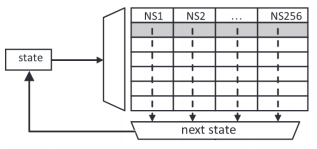
\includegraphics[width=0.4\textwidth]{../src/resources/table.png}}
            \caption{Transition table representation}
            \label{table}
        \end{figure}

        Untuk mengurangi kebutuhan terhadap penanda status akhir, nomor status akan disusun ulang. Status akhir akan diletakkan pada status pertama hingga ke-N. Sedangkan status lainnya termasuk status awal dimulai dari N+1. Dengan demikian, kebutuhan memori untuk penanda akan berkurang. Selain itu, operasi pengecekan dalam kode \emph{kernel} lebih sederhana dan ringan.

    \subsection{Alokasi \emph{Thread}}
        Meskipun \emph{thread} dibangkitkan sangat banyak, banyak juga diantara \emph{thread} yang akan berhenti sangat awal. Sehingga, muatan pencocokan tiap \emph{thread} dapat timpang cukup jauh dan utilisasi GPU rata-rata menjadi rendah. Untuk menunjang utilisasi GPU, \cite{lin2013} mengusulkan alokasi memori yang berulang.

        Dalam satu blok, satu atau beberapa \emph{byte stream} akan ditempatkan sebagai lokasi awal satu \emph{thread}. Misal, dalam blok berisi 4.096 \emph{byte} dengan 512 \emph{thread}, \emph{thread} pertama akan memulai pencocokan pada posisi kelipatan 512. Akibat dari penugasan yang berulang, secara statistik kemungkinan ketimpangan muatan dari masing-masing \emph{thread} akan berkurang \cite{lin2013}. 

    \subsection{Optimasi pada Memori GPU}
        Untuk memaksimalkan utilisasi GPU dan mengurangi latensi akibat transfer data, beberapa metode dapat diterapkan. Salah satu metode yang sangat umum adalah penggunaan \emph{shared memory}. \emph{Shared memory} memiliki latensi yang lebih kecil beberapa kali lipat dibandingkan \emph{global memory}. Namun, ukuran \emph{shared memory} sangat terbatas. Selain itu, \emph{shared memory} harus di-"replikasi" ke setiap \emph{block}. 

        Dengan memanfaatkan sifat \emph{early terminate} pada PFAC, penggunaan \emph{shared memory} dapat dihemat. Transisi dari \emph{state} awal akan selalu diakses namun kemungkinan pencocokan berhenti sangat tinggi \cite{lin2013}. Sehingga transisi ini akan dimuat ke \emph{shared memory} untuk menurunkan latensi ketika pembacaan tabel transisi.

        Sisa tabel transisi yang masih ada di \emph{global memory} akan ditingkatkan dengan \emph{texture memory}. Diantara keuntungan \emph{texture memory} adalah memiliki \emph{cache} yang lebih besar dan mampu melakukan transpolasi sehingga dapat memanfaatkan \emph{cache} untuk pola yang susah ditebak \cite{lin2013}. Kelemahan \emph{texture memory} data ditulis hanya dari \emph{host}, cocok dengan skema pencocokan yang melakukan kompilasi kamus sekali dalam satu \emph{rule group}.

        Metode lainnya yaitu dengan melakukan \emph{batching} dan menyimpan batch dalam \emph{pinned memory}. \emph{Pinned memory} adalah memori yang dialokasi di \emph{host} dan tidak dapat di-\emph{swap} ke disk. Penggunaan \emph{pinned memory} untuk \emph{buffer} input dapat menurunkan kemungkinan swappiness untuk ukuran \emph{buffer} yang besar. Selain itu, \emph{pinned memory} juga memungkinkan adanya DMA dari \emph{host} ke \emph{device} maupun sebaliknya \cite{gnort2008}.

        Penggunaan \emph{thread} per \emph{block} dibatasi sebesar 32 \emph{thread} untuk mencegah \emph{bank conflict}. Ukuran \emph{bank} pada \emph{shared memory} pada GPU NVIDIA 940MX yang memiliki arsitektur Maxwell yaitu 32. Jika akses ke \emph{shared memory} lebih besar dari ukuran \emph{bank}, operasi akan diserialisasi dan berdampak ke latensi secara signifikan \cite{lin2013}.

\section{Implementasi pada Snort}
    Dalam mengimplementasi modul pencocokan string, akan digunakan \emph{interface} MPSE (\emph{multi pattern search engine}). Modul deteksi pada Snort akan memuat semua kelas yang mengimplementasi \emph{interface} MPSE. Pilihan metode pencocokan akan diberikan dari konfigurasi sesuai definisi pada file header.

    \emph{Interface} MPSE sendiri berisi beberapa fungsi yang digunakan untuk analisis sebagaimana pada Tabel~\ref{mpse} berikut.

    \begin{table}[htbp]
    \caption{Fungsi yang diimplementasi}
    \begin{center}
    \begin{tabular}{|m{2cm}|m{5cm}|}
    \hline
    \rowcolor{gray!15}
    \textbf{Nama fungsi}& \textbf{Deskripsi} \\
    \hline
    \textit{init} & Menginisiasi struktur data dan melakukan alokasi \\
    \hline
    \textit{register} & Mendaftarkan pola ke dalam larik, sekaligus memperbarui jumlah \emph{state} maksimal \\
    \hline
    \textit{compile} & Membentuk kamus berdasarkan pola yang telah didaftarkan \\
    \hline
    \textit{match} & Melakukan pencocokan string ke kamus yang dibentuk \\
    \hline
    \textit{cleanup} & Melakukan dealokasi dan menghapus semua informasi pencocokan \\
    \hline
    \end{tabular}
    \label{mpse}
    \end{center}
    \end{table}

    Kemudian juga diimplementasi struktur data \emph{handle} yang akan menampung tabel dan larik yang diperlukan oleh MPSE. Isi dari \emph{handle} milik PFAC yaitu:

    \begin{enumerate}
        \item Larik untuk daftar pola yaitu \emph{array of string}
        \item Tabel transisi
        \item Tabel temporer untuk menampung daftar pola
        \item Larik untuk hasil pencocokan berupa \emph{array of integer}
        \item Jumlah \emph{state} maksimal
        \item Jumlah \emph{state} efektif
        \item Jumlah \emph{final state}
    \end{enumerate}

\section{Pengujian}
    \subsection{Strategi Pengujian}
        Pengujian dilakukan untuk mendapatkan perbandingan kinerja antara modul yang dikembangkan dan modul yang ada dalam NIDS Snort. Pengujian dibatasi dengan menggunakan konfigurasi \emph{data acquisition} PCAP dengan masukan \emph{file} tcpdump saja. Berkas didapatkan dari arsip DEFCON tahun 2017. \emph{Live testing} tidak diujikan dalam Tugas Akhir ini mengingat kapasitas \emph{network interface} dapat menjadi \emph{bottleneck} sehingga hasil perbandingan tidak akurat.

        Pengujian dilakukan pada komputer dengan spesifikasi seperti pada Tabel ~\ref{test-spec} berikut.
        
        \begin{table}[htbp]
            \caption {Spesifikasi Lingkungan Pengujian}
            \begin{center}
                \begin{tabular}{|l|l|}
                    \hline
                    \rowcolor{gray!15}
                    \textbf{Komponen} & \textbf{Spesifikasi} \\
                    \hline                    
                    Sistem Operasi & Ubuntu 16.04.5 amd64 \\
                    \hline                    
                    CPU & Intel Core i7-7500U CPU @ 2.70GHz × 4 \\
                    \hline                    
                    \emph{Host} RAM & 16 GB \\
                    \hline                    
                    Media Penyimpanan & SSD SATA III 6 Gbps \\
                    \hline                    
                    GPU & NVIDIA GeForce 940MX \\
                    \hline                    
                    Arsitektur GPU & Maxwell \\
                    \hline                    
                    \emph{Compute Capability} & 5.0 \\
                    \hline                    
                    \emph{Dedicated Video} RAM & 2 GB \\
                    \hline                    
                    CUDA \emph{Runtime} & CUDA 8.0 r2 \\
                    \hline                    
                    C/C++ \emph{Compiler} & GCC 5.4.0 \\
                    \hline                    
                    \end{tabular}
            \label{test-spec}
            \end{center}
        \end{table}

        Ada 5 skenario yang akan diujikan dalam penelitian ini: 
        \begin{enumerate}
        
            \item \emph{Baseline} (Aho-Corasick dengan \emph{multithreading} CPU) \\
            \emph{Baseline} akan menggunakan konfigurasi default Snort. Ini menjadi dasar pengukuran kinerja dan kebenaran program yang diimplementasikan pada GPU.

            \item Skenario 1 (PFAC dengan \emph{global memory}) \\
            Skenario ini adalah skenario paling dasar. Optimasi hanya dilakukan pada algoritma tanpa melibatkan optimasi pada latensi GPU.

            \item Skenario 2 (PFAC dengan \emph{shared memory}) \\
            Skenario ini memanfaatkan \emph{shared memory} untuk mengurangi akses ke \emph{global memory}. Transisi \emph{state} awal ke tiap huruf serta \emph{stream} masukan ditampung dalam \emph{shared memory}.

            \item Skenario 3 (PFAC dengan \emph{shared memory} dan \emph{pinned memory}) \\
            Skenario ini mirip dengan skenario 2 dengan tambahan \emph{pinned memory} pada \emph{buffer}. Mekanisme ini diharapkan dapat mengurangi \emph{swappiness} dan memungkinkan DMA (\emph{direct memory access}).

            \item Skenario 4 (PFAC dengan \emph{shared memory}, \emph{pinned memory}, dan \emph{texture memory}) \\
            Skenario ini mirip dengan skenario 3 dengan tambahan \emph{texture memory} pada kamus. Dengan \emph{cache} yang lebih besar, penggunaan \emph{texture memory} diharapkan mengurangi transfer memori.

        \end{enumerate}
        
    \subsection{Hasil Pengujian Kinerja}
        Pengujian dilakukan dengan menjalankan Snort dengan konfigurasi \emph{data acquisition} PCAP, yaitu membaca berkas PCAP dan menggunakan \emph{single thread} untuk implementasi GPU dan 4 \emph{thread} untuk implementasi bawaan Snort. \emph{Ruleset} yang digunakan yaitu Snort VRT 3000 yang didapat dari laman Snort. Pengujian dilakukan untuk ukuran \emph{buffer} yang bervariasi, yaitu 128 kB, 512 kB, 1024 kB, dan 2018 kB.

        \begin {table}[h]
\begin{center}
\caption {Hasil Pengujian}

    \begin{tabular}{|p{4cm}|p{4cm}|p{4cm}|}

    \hline
    \rowcolor{gray!10}
    Skenario & Runtime (detik) & Speedup \\
    \hline

    \emph{Baseline} & 94.631856 & 1 \\
    \hline
    
    Skenario 1 & 424.277725 & 0.21 \\
    \hline
    
    Skenario 2 & 265.578648 & 0.4 \\
    \hline
    
    Skenario 3 & 265.913109 & 0.4 \\
    \hline

    \end{tabular}

\end{center}
\end{table}
 

        Hasil skenario 1 memilki kapasitas paling rendah. Alasannya yaitu karena operasi pencocokan \emph{string} adalah operasi yang \emph{memory-bound}. Diperlukan banyak akses ke penyimpanan kamus untuk mendapatkan transisi ke \emph{next state}. Karena kamus disimpan di \emph{global memory}, maka \emph{fetch} ke \emph{global memory} menjadi sering dan menimbulkan latensi yang cukup besar.
        
        Skenario 2 secara umum lebih cepat beberapa kali daripada skenario 1, yaitu sekitar 15 kali lipat lebih cepat. Hal ini karena kecepatan akses \emph{global memory} lebih besar dari \emph{shared memory}. Dalam skenario ini, \emph{input string} seharusnya tidak berpengaruh banyak karena adanya \emph{coalescing access}. Sehingga pemuatan baris transisi dari \emph{state} awal ke \emph{shared memory} memiliki pengaruh yang besar terhadap \emph{throughput} sistem. Ini menunjukkan bahwa mayoritas \emph{thread} akan berhenti pada awal pencocokan.
        
        Skenario 3 tidak terlalu berpengaruh terhadap skenario 2. Keuntungan \emph{pinned memory} tidak terlalu terlihat bahkan cenderung memperlambat. Sejalan dengan eksperimen yang dilakukan \cite{gnort2008}. Ini karena \emph{pinned memory} memiliki \emph{overhead} saat alokasi dan dealokasi. Kemungkinan besar ini terjadi karena ukuran \emph{buffer} belum terlalu besar. \emph{Overhead} saat alokasi masih belum sebanding dengan perbedaan \emph{transfer} antara DMA dan melalui CPU. Selain itu, juga tidak terjadi \emph{swap} terhadap \emph{page} yang terdapat \emph{buffer} karena ukuran memori masih kecil.
        
        Sedangkan skenario 4 baru terlihat perbedaan signifikan terhadap skenario 2 dan 3 pada \emph{buffer} sebesar 1 MB ke atas. Terlihat bahwa adanya \emph{cache} pada memori tekstur membantu menurunkan akses ke memori global dan meningkatkan kinerja keseluruhan modul. 

\section{Kesimpulan}
 
    Peningkatan kinerja pencocokan string pada IDS Snort menggunakan GPU berhasil dilakukan dengan cara mengubah pendekatan algoritma yang digunakan agar memaksimalkan utilisasi GPU. Implementasi dilakukan berbasis teknik PFAC. Teknik ini memanfaatkan kemampuan GPU untuk membangkitakan banyak \emph{thread} serta \emph{memory coalescing} ketika mengakses karakter yang bersebelahan dalam \emph{stream}.    
    Operasi pencocokan string dari kamus merupakan operasi yang \emph{memory bound} sehingga dilakukan beberapa teknik untuk mengurangi \emph{latency gap} antara akses I/O, memori dan komputasi GPU. Di antara teknik yang digunakan yaitu penggunaan \emph{pinned memory} pada \emph{buffer input} dan \emph{texture memory} pada kamus. Selain itu, digunakan juga penggunaan \emph{shared memory} untuk menampung \emph{buffer input} dan tabel transisi dari \emph{state} awal untuk menghemat \emph{fetch} pada memori global.
    Parametrisasi dapat dilakukan pada ukuran \emph{buffer input}. Dengan menambah ukuran \emph{buffer input}, jumlah pengiriman paket dari \emph{host} ke \emph{device} dapat berkurang dan dapat menurunkan latensi secara drastis.

% \section{Acknowledgment}

\bibliography{references}
\bibliographystyle{IEEEtran}

\end{document}
